\documentclass{article}
\usepackage{cmap}
\usepackage[utf8]{inputenc}
\usepackage[english,ukrainian]{babel}
\usepackage{graphicx}
\usepackage{geometry}
\usepackage{listings}
\usepackage{float}
\usepackage{amsmath}
\geometry{
	a4paper,
	left=20mm,
	right=20mm,
	top=15mm,
	bottom=15mm,
}
\lstset{
	language=c,
	tabsize=4,
	keepspaces,
	showstringspaces=false,
}
\graphicspath{ {./pictures} }
\setlength{\parindent}{4em}

\newcommand\subject{Організація комп’ютерних мереж}
\newcommand\lecturer{асистент кафедри ПЗ \\ Задорожний І.М.}
\newcommand\teacher{асистент кафедри ПЗ \\ Задорожний І.М.}
\newcommand\mygroup{ПЗ-22}
\newcommand\lab{6}
\newcommand\theme{Дослідження роботи web-сервера та протоколу HTTP}
\newcommand\purpose{Ознайомитися основами протоколу HTTP, дослідити формат
	повідомлень HTTP}

\begin{document}
\begin{normalsize}
	\begin{titlepage}
		\thispagestyle{empty}
		\begin{center}
			\textbf{МІНІСТЕРСТВО ОСВІТИ І НАУКИ УКРАЇНИ\\
				НАЦІОНАЛЬНИЙ УНІВЕРСИТЕТ "ЛЬВІВСЬКА ПОЛІТЕХНІКА"}
		\end{center}
		\begin{flushright}
			\textbf{ІКНІ}\\
			Кафедра \textbf{ПЗ}
		\end{flushright}
		\vspace{200pt}
		\begin{center}
			\textbf{ЗВІТ}\\
			\vspace{10pt}
			до лабораторної роботи № \lab\\
			\textbf{на тему}: “\textit{\theme}”\\
			\textbf{з дисципліни}: “\subject”
		\end{center}
		\vspace{112pt}
		\begin{flushright}
			
			\textbf{Лектор}:\\
			\lecturer\\
			\vspace{28pt}
			\textbf{Виконав}:\\
			
			студент групи \mygroup\\
			Коваленко Д.М.\\
			\vspace{28pt}
			\textbf{Прийняв}:\\
			
			\teacher\\
			
			\vspace{28pt}
			«\rule{1cm}{0.15mm}» \rule{1.5cm}{0.15mm} 2023 р.\\
			$\sum$ = \rule{1cm}{0.15mm}……………\\
			
		\end{flushright}
		\vspace{\fill}
		\begin{center}
			\textbf{Львів — 2023}
		\end{center}
	\end{titlepage}
		
	\begin{description}
		\item[Тема.] \theme.
		\item[Мета.] \purpose.
	\end{description}

\section*{Теоретичні відомості}
Опишіть основні методи HTTP-запиту. 
\begin{itemize}
	\item Метод GET запитує вміст вказаного ресурсу.  
	\item Метод POST передає призначені для користувача дані (наприклад, з HTML-форми) заданому ресурсу.
	\item Метод HEAD – відрізняється від методу GET тим, що у відповіді сервера відсутнє тіло.
	\item Метод PUT – завантажує вказаний ресурс на сервер (на відміну від методу GET, який бере ресурс з сервера). 
	\item Метод PATCH – працює аналогічно PUT, тобто завантажує певну частину ресурсу на сервер, але на відміну від методу PUT він застосовується лише до фрагмента ресурсу. 
	\item Метод DELETE – видаляє вказаний ресурс. 
	\item Метод TRACE – повертає отриманий запит так, щоб клієнт зміг відстежити, що саме проміжні сервери додають або змінюють в запиті.
	\item Метод LINK– встановлює зв'язок даного ресурсу з іншими. 
	\item Метод UNLINK – розриває встановлений раніше зв'язок даного ресурсу з іншими.
	\item Метод CONNECT – використовується для встановлення захищеного з'єднання через нешифрований проксі. 
	\item Метод OPTIONS – використовується для визначення можливостей веб-сервера або параметрів з’єднання для конкретного ресурсу. Сервер у відповідь включає заголовок Allow зі списком методів, які він підтримує. Замість URI при методі OPTIONS записується символ “*”.
\end{itemize}

Поясніть призначення URI.

URI (Uniform Resource Identifier, уніфікований ідентифікатор ресурсу) –
це символьний рядок, що ідентифікує ресурс (документ, зображення, файл,
електронну поштову скриньку тощо). Основне призначення таких
ідентифікаторів — зробити можливою взаємодію з представленнями ресурсів
через мережу, використовуючи спеціальні протоколи. URI визначається
схемами, які визначають синтаксис та відповідні протоколи. Найбільш
поширеною формою URI є уніфікований локатор ресурсів (URL), який
неофіційно називають веб-адресою. Рідше використовується уніфіковане ім'я
ресурсів (URN), яке було розроблене, щоб доповнити URL забезпеченням
механізму для ідентифікації ресурсів в просторі імен.

Для чого використовується заголовок Expires? Наведіть приклади.

Expires - використовується у механізмі кешування. У ньому
повідомляється термін придатності представлених у відповіді даних. У
значенні вказується дата і час за Гринвічем (у форматі RFC 1123), після
закінчення яких кеш повинен вважатися застарілим, а запити перенаправлятися
на сервер-джерело для перевірки його актуальності або отримання новішої
відповіді.

Наприклад: Expires: Mon, 18 Oct 2010 14:15:00 GMT.

\section*{Хід виконання}
\begin{figure}[H]
	\centering
	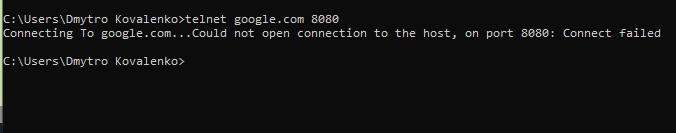
\includegraphics[width=\textwidth]{11}
\end{figure}

\begin{figure}[H]
	\centering
	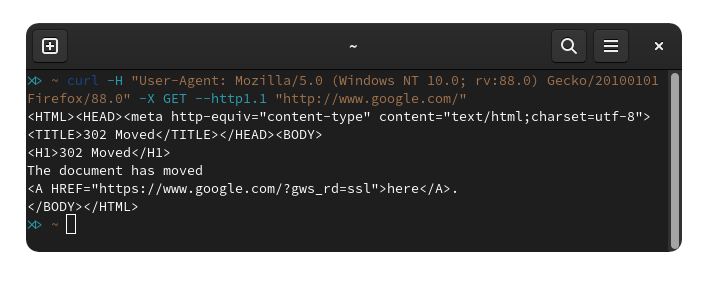
\includegraphics[width=\textwidth]{21}
\end{figure}
\begin{figure}[H]
	\centering
	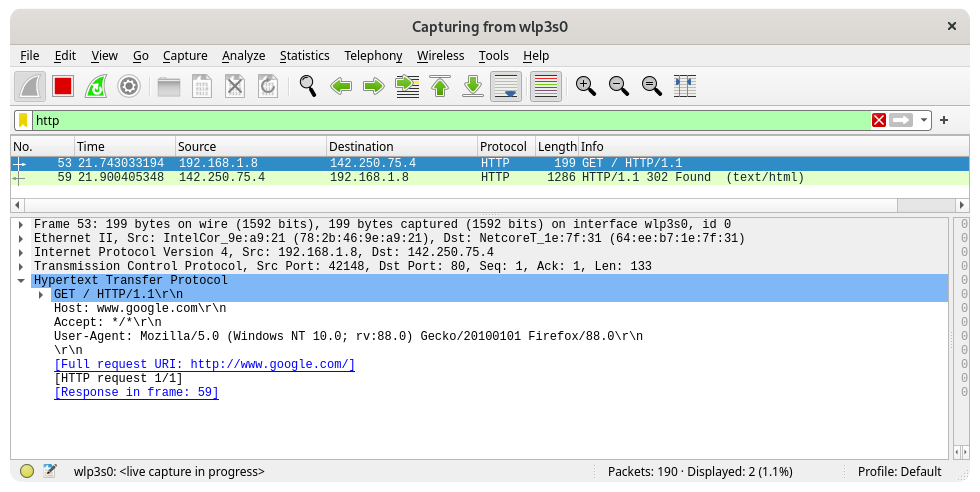
\includegraphics[width=\textwidth]{22}
\end{figure}

\begin{figure}[H]
	\centering
	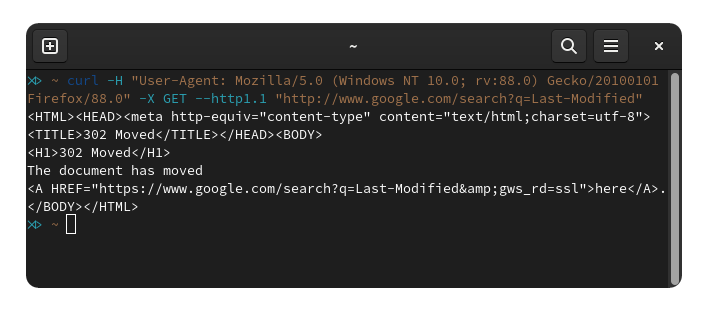
\includegraphics[width=\textwidth]{31}
\end{figure}
\begin{figure}[H]
	\centering
	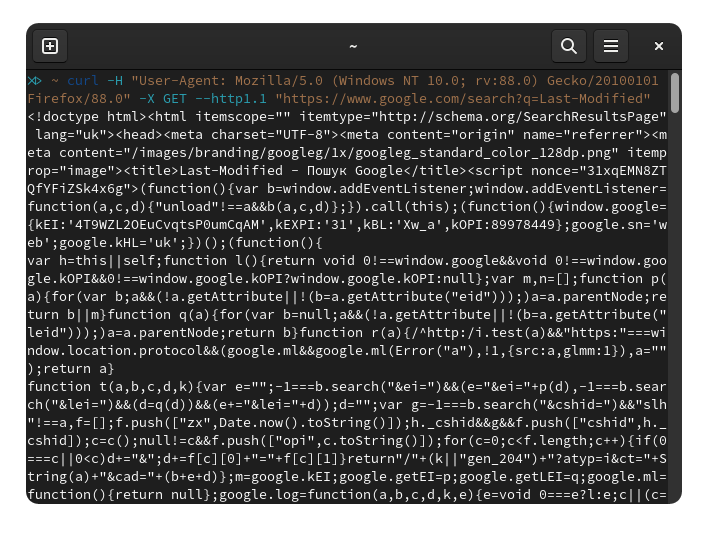
\includegraphics[width=\textwidth]{32}
\end{figure}
\begin{figure}[H]
	\centering
	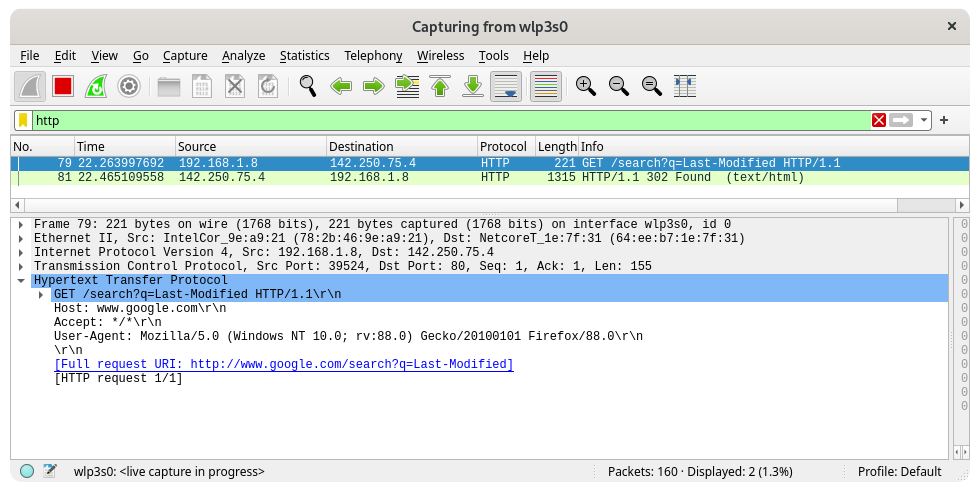
\includegraphics[width=\textwidth]{33}
	\caption{HTTP запит}
\end{figure}
\begin{figure}[H]
	\centering
	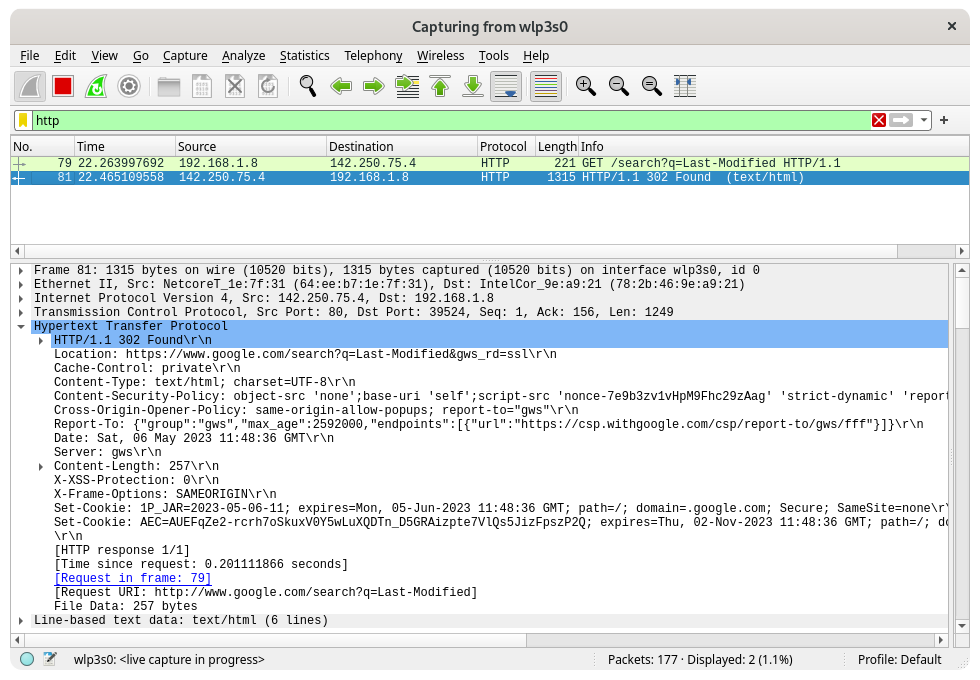
\includegraphics[width=\textwidth]{34}
	\caption{HTTP відповідь}
\end{figure}

\begin{figure}[H]
	\centering
	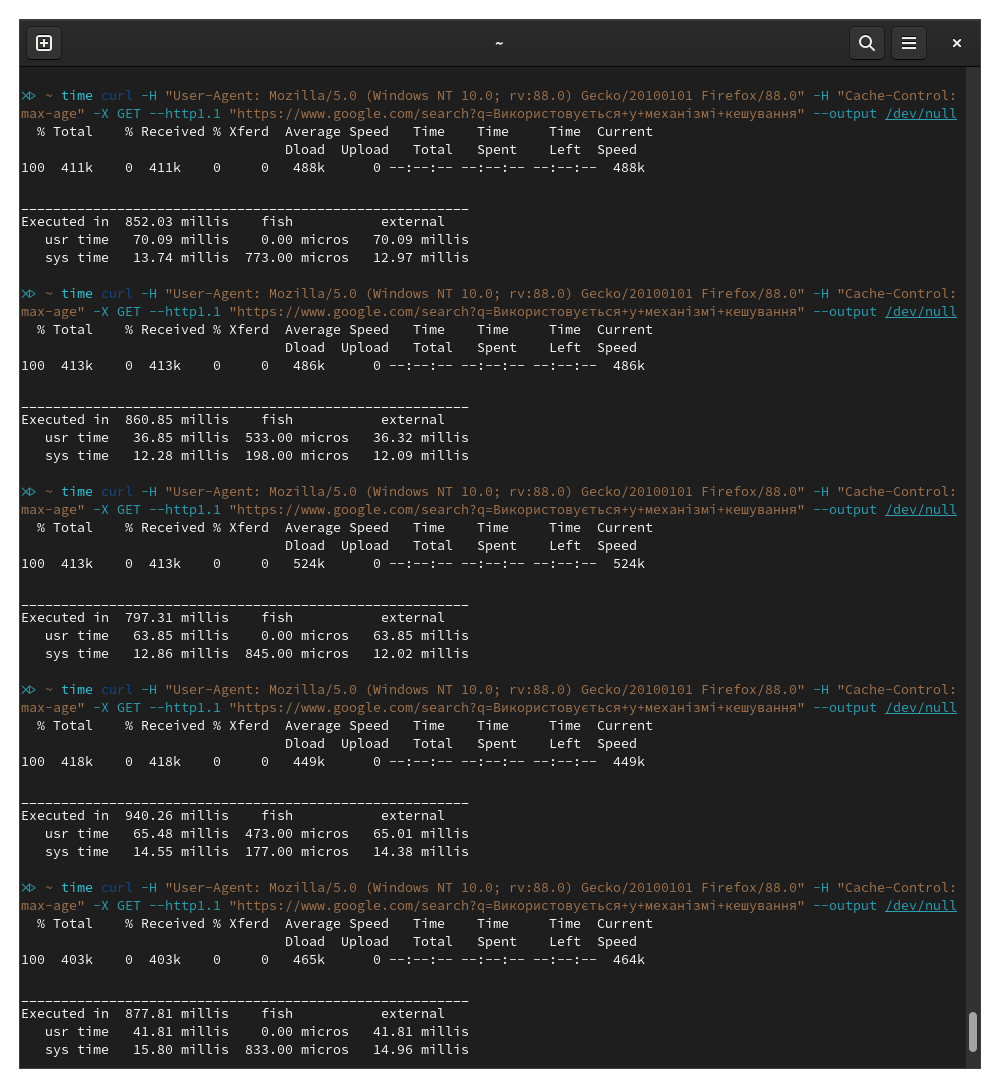
\includegraphics[width=\textwidth]{43}
	\caption{Надсилання запитів з кешуванням}
\end{figure}
\begin{figure}[H]
	\centering
	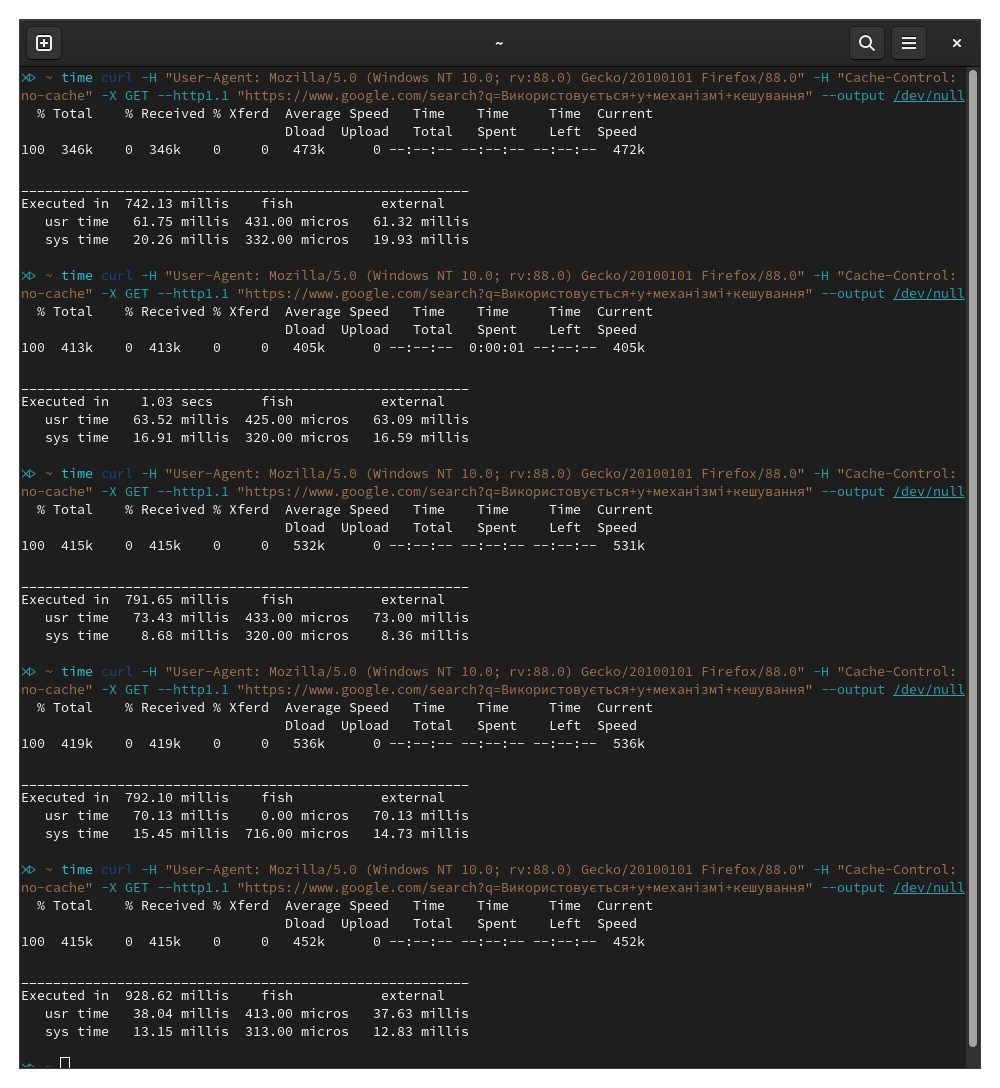
\includegraphics[width=\textwidth]{44}
	\caption{Надсилання запитів без кешування}
\end{figure}
\begin{figure}[H]
	\centering
	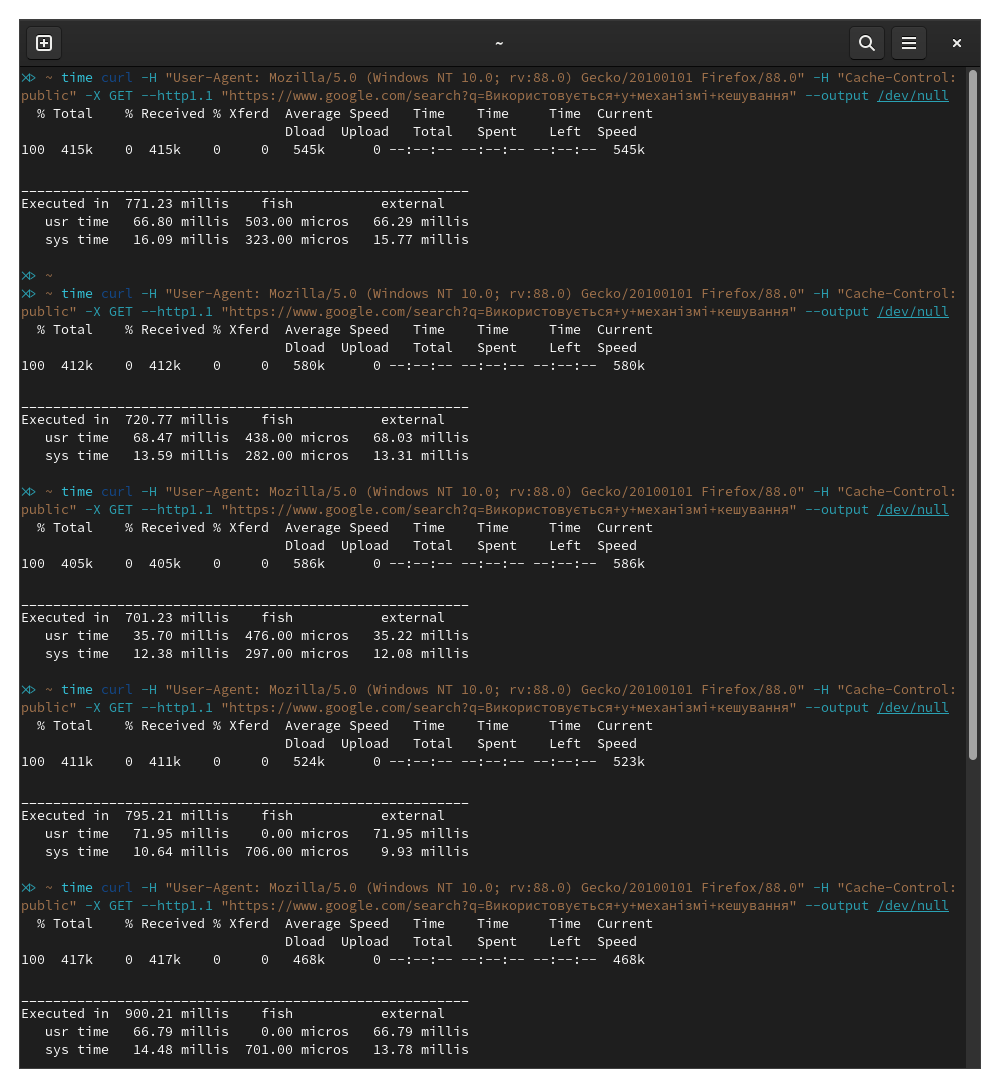
\includegraphics[width=\textwidth]{45}
	\caption{Надсилання запитів з кешуванням з директивою відповідно до варіанту}
\end{figure}
\begin{figure}[H]
	\centering
	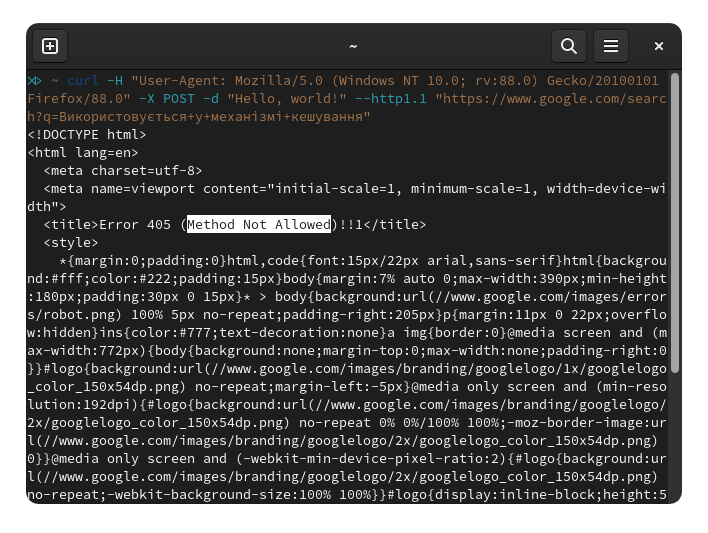
\includegraphics[width=\textwidth]{46}
\end{figure}

\section*{Висновки}
Під час виконання лабораторної роботи я ознайомився основами протоколу HTTP, дослідити формат
повідомлень HTTP.
	    
\end{normalsize}
\end{document}
